%!TEX root = ../report_template.tex
\section{Results and Discussion}
% Todo Introduction
As it is introduced in TODO SEC the student-to-teacher ratio can be compared to Abitur grades, repeaters and budgets. Importantly, the Abitur grades can only be analyzed for the German average, due to the missing representation. In contrast, the repeaters and budgets are analyzed for each federal state. 

One of the key findings of this analysis is the strong correlation between the average grades across all federal states and the student-to-teacher ratio for German grammar schools. As shown in \autoref{fig:regression-stt-grade}, the relationship between both is nearly linear. In addition, the result contains neither clusters nor outliers. Hence, a smaller student-to-teacher ratio strongly correlates to better Abitur grades with a Pearson correlation coefficient of $0.98$.

\begin{figure}[ht]
    \centering
    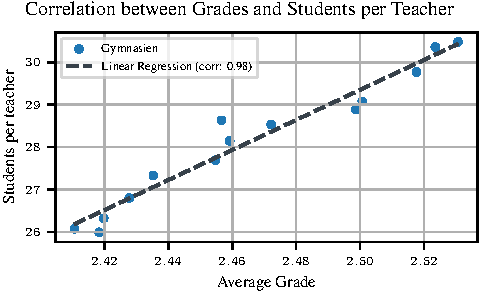
\includegraphics{fig/fig_correlation_grades_students_per_teacher.pdf}
    \caption{Linear regression on the student-to-teacher ratio by average Abitur grade. The resulting regression line (\textcolor{TUred}{\rule[-0.2ex]{0.5em}{2pt} \rule[-0.2ex]{0.5em}{2pt}}) is calculated over the aggregated average overall grammar schools (\textcolor{TUlightblue}{\tikz\draw[fill={TUlightblue}] (0,0) circle (0.25em);}) in Germany.}
    \label{fig:regression-stt-grade}
\end{figure}

This result confirms the initial hypothesis of the big influence of the student-to-teacher ratio and is consistent with studies in other countries \cite{kasau_onesmus_mulei_pupil-teacher_2016,koc_impact_2015,dickson_economic_1984}. 

% TODO: Put at the end
% Since the student-teacher ratio got smaller in recent years and the grades went on a steep increase, this observation and the strong correlation underline the necessity of having enough teaching personnel available.

However, the Abitur grades give only an insight into grammar schools. Thus, the correlation with repeaters and budgets are shown in \autoref{fig:heatmap_correlation_students_per_teacher_repeaters_budget}. It presents a visualization of the Pearson correlation coefficients, analyzing the relationship between the number of children per teacher and the average number of repeaters, as well as the educational budget per child. Therefore, the Pearson correlation coefficients for each state are normalized to the used color map scale.

\begin{figure}[ht]
    \centering
    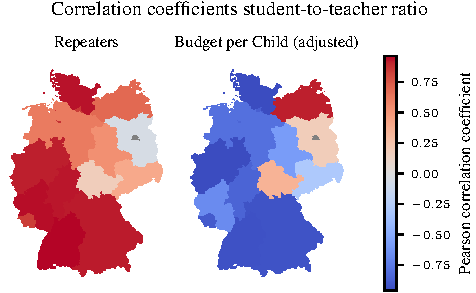
\includegraphics{fig/fig_heatmap_correlation_students_per_teacher_repeaters_budget.pdf}
    \caption{Pearson correlation coefficients between the student-to-teacher ratio and the relative repeater count (left) and the inflation-adjusted average budget per child (right). \textcolor{red}{Red} indicates positive, \textcolor{gray}{light gray} neutral, \textcolor{TUdark}{gray} missing, and \textcolor{blue}{blue} negative correlations between the variables.}
    \label{fig:heatmap_correlation_students_per_teacher_repeaters_budget}
\end{figure}

% Todo better sentence
As shown in \autoref{fig:heatmap_correlation_students_per_teacher_repeaters_budget}, there is a strong positive and negative correlation between the student-to-teacher ratio and the number of repeaters and budget per child respectively for the most federal states. Interestingly, there is a big difference between \emph{old} and \emph{new} federal states for both correlations. Especially, the correlations for Thüringen and Brandenburg differ from the other states for both and for Mecklenburg Vorpommern for the budget.

% TODO Source
% After seeing this visualisation, suggesting that schools simply require additional funding to hire more teachers might seem like a straightforward solution. The data from Thüringen, Mecklenburg-Vorpommern, and Brandenburg shows that this is not the case. For them, the correlation between budget and students per teacher is positive.
The difference between the federal states can be explained by an increase in the number of students over the past decade in the new federal states \cite{thuringer_ministerium_fur_bildung_jugend_und_sport_verteilung_2023, brandenburger_ministerium_fur_bildung_jugend_und_sport_zahlen_2023,statistisches_amt_mecklenburg-vorpommern_statistik_nodate}. Since the budget per child stays the same and increases in all states\footref{footnote:budget}, the schools get more money in total. This results in more vacancies at schools and other investments, like digitalization and maintenance of schools (TODO). The problem is that there have been more vacancies than prospective teachers in recent years \cite{kultusminister_konferenz_lehrkrafteeinstellungsbedarf_2023}. As the analysis\footref{footnote:teachers-children} shows, this leads the schools employ more teachers in full-time, then in part-time. This results in a higher student-to-teacher ratio with the same budget.

% TODO Source
In contrast, the anomaly for the repeaters involves more aspects of the educational system, like the different curricula or conditions to repeating a class (TODO). Hence, an complete explanation for this results involves more datasets and effects, which are not analyzed in this paper.
% Possible explanation: In Bayern and Badenwürttemberg repeat with bad grades, In contrast in the norther states only if you want to.

% This below may already be conclusion

% Todo better citation
For every other of the 16 federal states, there is a very strong positive correlation, for the number of repeaters. This can be interpreted as meaning that the sufficient availability of teachers not only increases grades but is especially beneficial for challenged students. In contrast, a higher budget only helps when the schools can find teachers to employ. Making sure that many teachers are available is one of the most important challenges for the education system. The prognosis of the Kultusministerkonferenz \cite{kultusminister_konferenz_lehrkrafteeinstellungsbedarf_2023} shows that there are still more open positions than teachers that can fill them. Unfortunately, they predict that this gap will eventually close in the coming decade. This means that a further increase in grades in the future can be expected.

It is important to note that having enough teachers is not the only factor responsible for the rising Abitur grades. Nonetheless, it is one of the most important ones. While the German education system faces several challenges, our demonstration illustrates that it has effectively addressed certain issues over the past decade and is poised to continue resolving them in the future. The increasing grades are a result of an increase in the competence of the students, facilitated by an improvement in the education system, especially a decrease in the student-teacher ratio.
